\title{Homework 5 Report}
\author{
        Hooley Cheng \\
                Department of Mathematics\\
        University of Washington\\
        Seattle, WA, 98105, U.S.
           
}
\date{\today}

\documentclass[12pt]{article}

\usepackage{hyperref}
\usepackage{amsmath}
\usepackage{graphicx}
\usepackage{float}
\usepackage{listings}

\usepackage{titlesec}
\begin{document}
\maketitle

\begin{abstract}
In this assignment, we are going to build an efficient neural network that helps us to classify Fashion MNIST.
\end{abstract}

\section{Introduction and Overview}\
The Fashion-MNIST data has 60000 different 28 * 28 images of fashion items, and each of them are marked with one class. For example:
\begin{figure}[H]
\begin{tabular}{cc}
  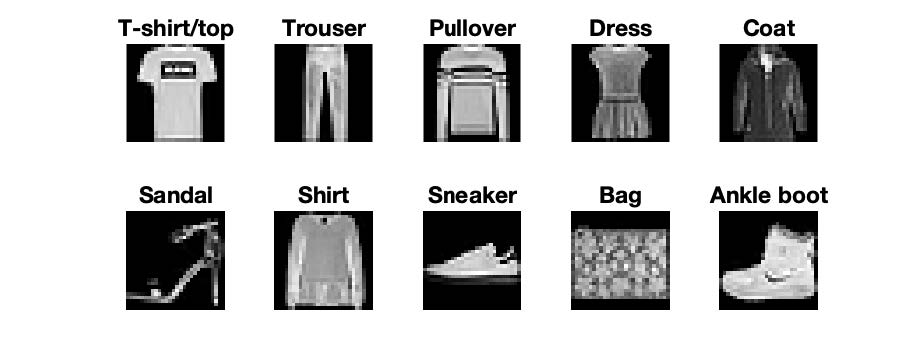
\includegraphics[width=\textwidth]{fashion.jpg}
\end{tabular}
\end{figure}
And we are going to investigate and discuss several structures of NN with high accuracy and generalization.

\section{Theoretical Background}
\subsection{Supervised Learning}
Supervised learning is the machine learning task of learning a function that maps an input to an output based on example input-output pairs. It infers a function from labeled training data consisting of a set of training examples. In supervised learning, each example is a pair consisting of an input object and a desired output value . A supervised learning algorithm analyzes the training data and produces an inferred function, which can be used for mapping new examples. An optimal scenario will allow for the algorithm to correctly determine the class labels for unseen instances. This requires the learning algorithm to generalize from the training data to unseen situations in a "reasonable" way.
\subsection{Artificial Neural Network}
Artificial neural networks are computing systems vaguely inspired by the biological neural networks that constitute animal brains. Such systems "learn" to perform tasks by considering examples, generally without being programmed with task-specific rules. \\
It is based on a collection of connected units or nodes called artificial neurons, which loosely model the neurons in a biological brain. Each connection, like the synapses in a biological brain, can transmit a signal to other neurons. An artificial neuron that receives a signal then processes it and can signal neurons connected to it.\\
In ANN implementations, the "signal" at a connection is a real number, and the output of each neuron is computed by some non-linear function of the sum of its inputs. The connections are called edges. Neurons and edges typically have a weight that adjusts as learning proceeds. The weight increases or decreases the strength of the signal at a connection. Neurons may have a threshold such that a signal is sent only if the aggregate signal crosses that threshold. Typically, neurons are aggregated into layers. Different layers may perform different transformations on their inputs. Signals travel from the first layer (the input layer), to the last layer (the output layer), possibly after traversing the layers multiple times.\\
\begin{figure}[H]
\begin{tabular}{cc}
  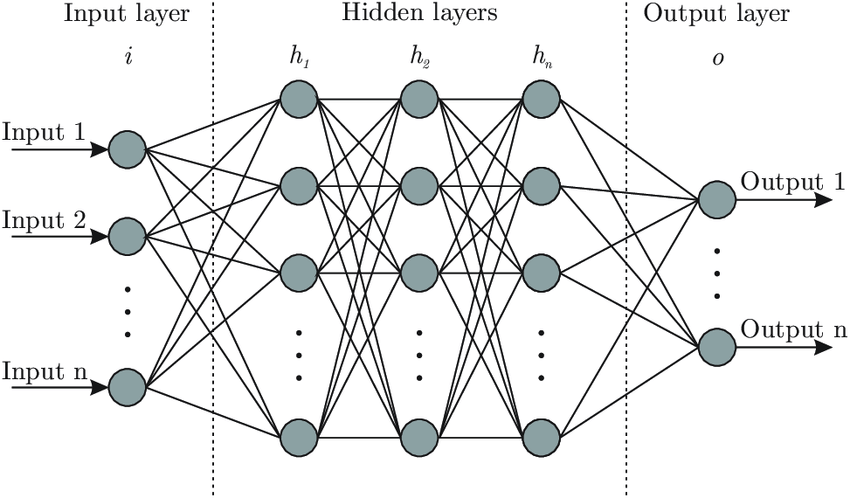
\includegraphics[width=\textwidth]{ann.png}
\end{tabular}
\end{figure}

\subsection{Convolutional Neural Network}
CNNs are regularized versions of multilayer perceptrons. Multilayer perceptrons usually mean fully connected networks, that is, each neuron in one layer is connected to all neurons in the next layer. The "fully-connectedness" of these networks makes them prone to overfitting data. Typical ways of regularization include adding some form of magnitude measurement of weights to the loss function. CNNs take a different approach towards regularization: they take advantage of the hierarchical pattern in data and assemble more complex patterns using smaller and simpler patterns. Therefore, on the scale of connectedness and complexity, CNNs are on the lower extreme.
\begin{figure}[H]
\begin{tabular}{cc}
  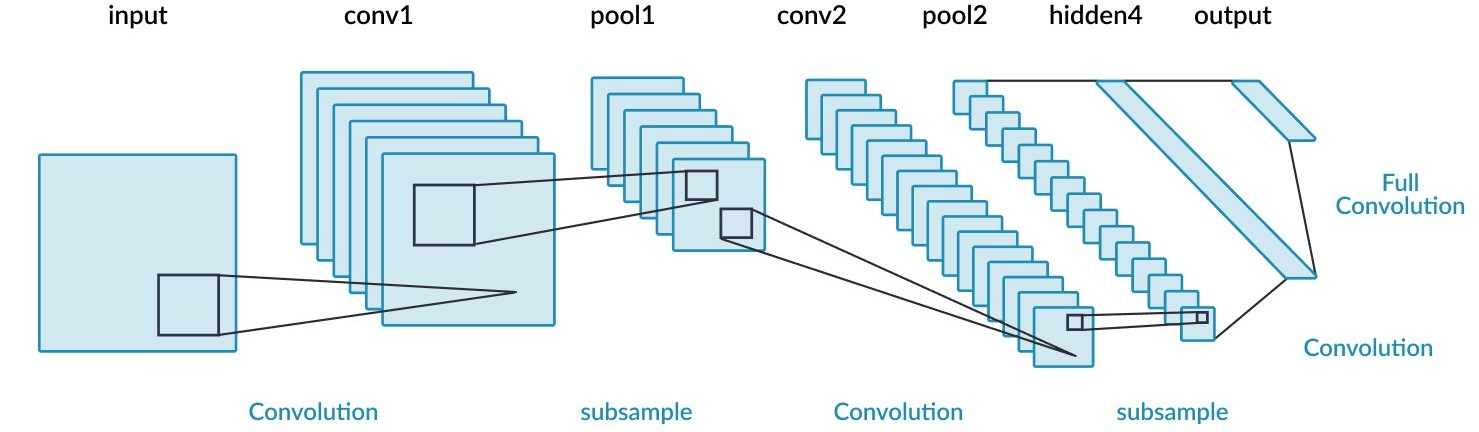
\includegraphics[width=\textwidth]{cnn.jpg}
\end{tabular}
\end{figure}

\section{Algorithm Implementation and Development}
\subsection{Fully Connected Neural Network Implementation}
First, we are going to try the classical neural network. We first construct our model to be 2 fully connected layers with 128 neurons in input layer and 10 neurons in output layer, and with ReLU activation function in all neurons. And we decided to use AdamBoost optimization which has auto-adaptive learning rate, and Sparse Categorical Cross-entropy as our loss function which has been shown to be the best choice for multi-class classification.
\begin{figure}[H]
\begin{tabular}{cc}
  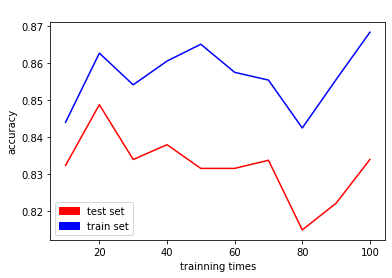
\includegraphics[width=\textwidth]{nn-1.png}
\end{tabular}
\end{figure}
As show in the figure, there is a little "back and forth" during training which is a clear signal of overshooting. Therefore, we might need to normalize our data with L2 norm and axis on 0. This will help our optimization to adapt its learning rate and preventing overshooting:
\begin{figure}[H]
\begin{tabular}{cc}
  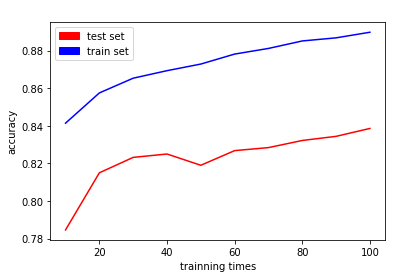
\includegraphics[width=\textwidth]{nn-3.png}
\end{tabular}
\end{figure}
Moreover, the accuracy at the end is about 0.87, which is a clear sign of underfitting. Therefore, we decided to add one hidden layer with 128 ReLU neurons. Since now our NN is much more complicated, its reasonable to also concern about overfitting. So, we also decided to add regularization to our network:\\
\begin{figure}[H]
\begin{tabular}{cc}
  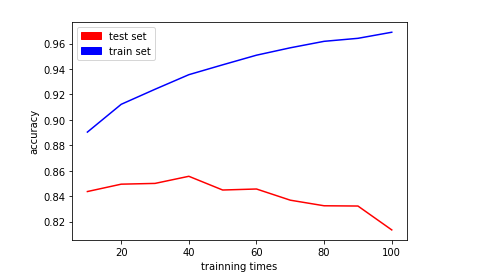
\includegraphics[width=\textwidth]{nn-4.png}
\end{tabular}
\end{figure}
However, the divergence of red and blue lines are clear signal of overfitting, even though we already add regularizations to each layer.
\subsection{Convoluntional Neural Network Implementation}
Due to the limitation of the classical neural network, we then decided to try another popular NN, which is called convolutional neural network and is been wildly used for image classification. Since finding an appropriate structure is very time-consuming, we decided to imitate a famous CNN called AlexNet as our starter point. Since we has much smaller input data size, we reduced filter numbers and layer depth of AlexNet but loosely keep the ratio and layout.
\begin{figure}[H]
\begin{tabular}{cc}
  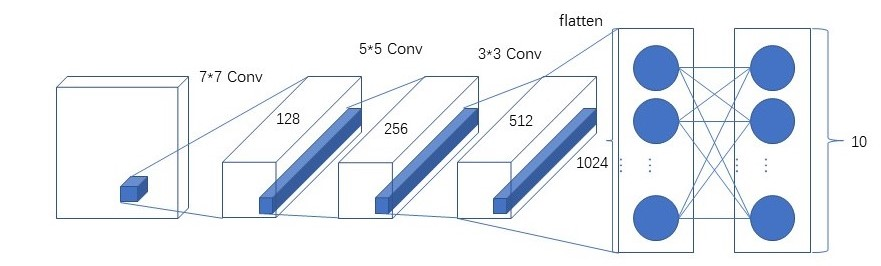
\includegraphics[width=\textwidth]{cnn-1.jpg}
\end{tabular}
\end{figure}
\section{Computational Results}
\subsection{Fully Connected Neural Network}
As we mentioned above, we have tried several different hyperparamenters to settle our final network, and its accuracy on validation data is 0.84.
\subsection{Convolutional Neural Network}
Before we actually got the outcome, we have decided to train 1000 times on each vector in the data set since we were considering that CNN might be more promising than classical NN. However, we get a very similiar outcome to that one with tons of times of training and much deeper network and careful tuned hyperparameter. The accuracy of our CNN on validation set is about 0.86.
\\
\\
*Unfortunately, training and tuning this CNN had already approached the limitation of our GPU, hence we sadly decided to stop investigating further on it.
\section{Summary and Conclusions}
Technically, CNN should work better than classical NN for image classification. However, we did not notice that phenomenon. This might because the image is too small that CNN cannot even take the advantage of extracting details. And also, the Universal Approximation Theorem tells us that with limited depth and number of neurons, a classical NN can approximate any function with arbitrary precision. Therefore, CNN might only be a best way to process high dimensional data than NN but not outstandingly more "intelligent" than it.
\section{Appendix A}
Tensorflow API Documentaion See:\\
 \url{https://www.tensorflow.org/api_docs}
\section{Appendix B: Matlab Source Code}
\section{python codes}
First NN model
\begin{verbatim}
model = tf.keras.Sequential([
    tf.keras.layers.Flatten(input_shape=(28, 28)),
    tf.keras.layers.Dense(128, activation='relu'),
    tf.keras.layers.Dense(10)
])

model.compile(optimizer='adam',
              loss=tf.keras.losses.SparseCategoricalCrossentropy(
              from_logits=True),
              metrics=['accuracy'])
\end{verbatim}
Second NN model
\begin{verbatim}
x_train_norm = tf.keras.utils.normalize(x_train, axis=0, order=2)
x_valid_norm = tf.keras.utils.normalize(x_valid, axis=0, order=2)
model = tf.keras.Sequential([
    tf.keras.layers.Flatten(input_shape=(28, 28)),
    tf.keras.layers.Dense(128, activation=tf.nn.relu, 
                          kernel_initializer
                          =tf.keras.initializers.RandomUniform(minval=-1,
                          maxval=1, seed=None)),
    tf.keras.layers.Dense(10, activation=tf.nn.sigmoid,
                          kernel_initializer
                          =tf.keras.initializers.RandomUniform(minval=-1,
                          maxval=1, seed=None)),
])

model.compile(optimizer='adam',
              loss=tf.keras.losses.SparseCategoricalCrossentropy(
              from_logits=True),
              metrics=['accuracy'])
\end{verbatim}
Third NN model
\begin{verbatim}
lamba = 0.01

x_train_norm = tf.keras.utils.normalize(x_train, axis=0, order=2)
x_valid_norm = tf.keras.utils.normalize(x_valid, axis=0, order=2)
model = tf.keras.Sequential([
    tf.keras.layers.Flatten(input_shape=(28, 28)),
    tf.keras.layers.Dense(128, activation=tf.nn.relu,
    activity_regularizer=tf.keras.regularizers.l2(lamba), 
                          kernel_initializer
                          =tf.keras.initializers.RandomUniform(minval=-1,
                          maxval=1, seed=None)),
    tf.keras.layers.Dense(128, activation=tf.nn.relu,
    activity_regularizer=tf.keras.regularizers.l2(lamba),
                          kernel_initializer
                          =tf.keras.initializers.RandomUniform(minval=-1,
                          maxval=1, seed=None)),
    tf.keras.layers.Dense(10, activation=tf.nn.sigmoid,
    kernel_regularizer=tf.keras.regularizers.l2(lamba),
                          kernel_initializer
                          =tf.keras.initializers.RandomUniform(minval=-1,
                          maxval=1, seed=None)),
])

model.compile(optimizer='adam',
              loss=tf.keras.losses.SparseCategoricalCrossentropy(
              from_logits=True),
              metrics=['accuracy'])
\end{verbatim}
CNN model
\begin{verbatim}
model = tf.keras.Sequential([
    tf.keras.layers.Conv2D(128, (7, 7), activation='relu', 
    input_shape=(28, 28, 1)),
    tf.keras.layers.MaxPool2D((2,2), padding='same'),
    tf.keras.layers.Conv2D(256, (5, 5), activation='relu'),
    tf.keras.layers.MaxPool2D((2,2), padding='same'),
    tf.keras.layers.Conv2D(512, (3, 3), activation='relu'),
    tf.keras.layers.MaxPool2D((2,2), padding='same'),
    tf.keras.layers.Flatten(),
    tf.keras.layers.Dense(1024, activation='relu'),
    tf.keras.layers.Dense(10, activation='softmax'),
])

model.compile(optimizer=tf.keras.optimizers.Adam(),
              loss=tf.keras.losses.SparseCategoricalCrossentropy(
              from_logits=True),
              metrics=['accuracy','sparse_categorical_accuracy'])

h = model.fit(x_train, y_train, epochs=1000, verbose=1,
validation_data=(x_valid_norm, y_valid))
test_loss, test_acc = model.evaluate(x_valid,  y_valid, verbose=2)
train_loss, train_acc = model.evaluate(x_train,  y_train, verbose=2)
\end{verbatim}
\end{document}